\section{Series de Tiempo}

\theoremstyle{definition}
\newtheorem{definicion}{Definición}

\subsection*{Definición Informal}
En términos informales, una serie de tiempo es un conjunto de datos recolectados secuencialmente en el tiempo. Este tipo de datos se dan en varios campos de estudio, como por ejemplo Economía, Ciencias de la Atmósfera, y otros.

Ejemplos de series de tiempo:

\begin{itemize}
    \item Volumen de lluvias en sucesivos días de un año
    \item Precio de acciones en diferentes meses
    \item Cantidad de habitantes de una ciudad año a año
\end{itemize}

\begin{figure}
\centering
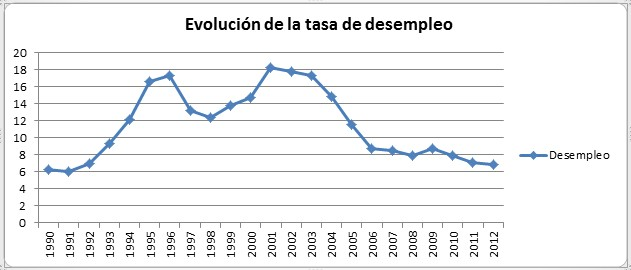
\includegraphics[width=15cm]{images/desocupacion.jpg}
\caption{Gráfico de serie de tiempo de la evolución del desempleo en Argentina \label{desocupacion}}
\end{figure}


\subsection*{¿Para qué queremos series de tiempo?}

Hay varios motivos por los cuales uno querría efectuar un análisis de una serie de tiempo.

\emph{1) Descripción} Usualmente, lo primero que se hace al obtener la serie de tiempo es graficarla y obtener las características más notorias de ésta. Por ejemplo, en \ref{desocupacion} puede notarse que hay una tendencia decreciente del $2003$ hasta el $2012$. En otras (como en el volumen de lluvias) podrá observarse cierta estacionalidad en la serie.

Si bien ésto no requiere técnicas avanzadas de análisis, es el primer paso fundamental para comprender una serie de tiempo.


\emph{2) Explicación} Cuando analizamos dos o más series de tiempo, podemos querer ver cómo se comportan en conjunto. Una variación en una serie de tiempo puede producir un cambio en otra. Por ejemplo, podemos intentar buscar como varían en conjunto la temperatura diaria con la cantidad de mL de lluvia caídos.

\emph{3) Predicción} Dada una serie de tiempo, podemos querer intentar predecir un valor futuro.

\emph{4) Control} Dado un proceso del que se mide cierto parámetro de calidad, podemos querer ajustar variables de entrada para mantenerla en ciertos valores.

En nuestro caso, nos es de interés 1 y 2.


\subsection{Procesos estocásticos}

\begin{definicion}
Una proceso estocástico es una colección de variables aleatorias $\{X_t \}_{t \in T}$ donde $T$ es un conjunto de puntos de tiempo. En nuestro caso, nos interesa $T = \mathbb{N}$, de manera que el proceso será de la forma $X_1, X_2, \ldots $
\end{definicion}

Podemos entender un proceso estocástico como un conjunto de variables ordenadas por el tiempo. Llamamos serie de tiempo a una observación de este proceso estocástico. Usualmente sólo tendremos esta instancia, a diferencia de otros problemas estadísticos donde tendremos muchas observaciones.


\subsection{Estacionariedad}

Un concepto importante en series de tiempo es el de estacionariedad. En lenguaje coloquial, una serie de tiempo estacionaria es aquella en la que no observamos cambios sistemáticos de ésta en el tiempo: si tomamos una parte de la serie, y observamos otro parte distinta de la serie, las propiedades de ésta se mantienen.

Ejemplos de series de tiempo estacionarias son las de ruido blanco, y ejemplos de no estacionarias aquellas que tienen una tendencia. (mejorar esto...)

\begin{definicion}
Un proceso estocástico $X_i, i \in \mathbb{N}$ se dice fuertemente estacionario si, para todo conjunto de índices $t_1, \ldots , t_n$ y para un desplazamiento $\tau \in \mathbb{N}$ tenemos que

\begin{displaymath}
    F_{X_{t_1}, X_{t_2}, \ldots , X_{t_n} } = F_{X_{t_1} + \tau, X_{t_2} + \tau, \ldots , X_{t_n} + \tau}
\end{displaymath}

Es decir, que la función de probabilidad se preserva por traslados.
\end{definicion}

Se derivan como propiedades que, para todo $X_t$ y cualquier desplazamiento $\tau$

\begin{align}
    E[X_t] &= E[X_{t + \tau}] \label{eq:1} \\
    Var[X_t] &= Var[X_{t + \tau}] \label{eq:2} \\
    Cov(X_s, X_t) &= Cov(X_{s+\tau}, X_{t + \tau}) \label{eq:3}
\end{align}

Las ecuaciones \ref{eq:1} y \ref{eq:2} nos dicen que tanto la media como la varianza son constantes (no dependen de $t$), y que la covarianza sólo depende de la diferencia $| s - t |$.


\begin{definicion}
    Un proceso se dice débilmente estacionario si cumple \ref{eq:1}, \ref{eq:2}, \ref{eq:3}
\end{definicion}

A partir de aquí, cuando hablemos de series estacionarias estaremos hablando de series débilmente estacionarias

